% ============================================================================
%  GAHIB — Research Highlights & Key Questions
%  A standalone companion document to accompany the main manuscript.
%
%  Target: Journal of King Saud University — Computer and Information
%          Sciences (JKSUCI)
% ============================================================================
\documentclass[11pt,a4paper]{article}

% ── Packages ──────────────────────────────────────────────────────────────
\usepackage[T1]{fontenc}
\usepackage{lmodern}
\usepackage{microtype}
\usepackage{xcolor}
\usepackage{hyperref}
\usepackage{geometry}
\usepackage{enumitem}
\usepackage{titlesec}
\usepackage{fancyhdr}
\usepackage{tikz}
\usepackage{parskip}
\usepackage{amssymb}
\usetikzlibrary{shadows.blur,calc,backgrounds}

% ── Page geometry ─────────────────────────────────────────────────────────
\geometry{
  left=2.4cm, right=2.4cm,
  top=1.8cm, bottom=1.8cm,
}

% ── Colour palette ────────────────────────────────────────────────────────
\definecolor{accentblue}{HTML}{1A5276}
\definecolor{ruleblue}{HTML}{2980B9}
\definecolor{deepteal}{HTML}{117864}
\definecolor{sunstone}{HTML}{B9770E}
\definecolor{coral}{HTML}{C0392B}
\definecolor{plum}{HTML}{6C3483}
\definecolor{lightgray}{HTML}{F2F2F2}
\definecolor{darkgray}{HTML}{4A4A4A}
\definecolor{softmist}{HTML}{F4F8FB}
\definecolor{questionbg}{HTML}{EBF5FB}
\definecolor{questionborder}{HTML}{2E86C1}
\definecolor{highlightbg}{HTML}{FEF9E7}
\definecolor{highlightborder}{HTML}{B9770E}

% ── Hyperlinks ────────────────────────────────────────────────────────────
\hypersetup{
  colorlinks=true,
  linkcolor=accentblue,
  urlcolor=ruleblue,
  pdfauthor={},
  pdftitle={GAHIB — Research Highlights & Key Questions},
}

% ── Header / footer ──────────────────────────────────────────────────────
\pagestyle{fancy}
\fancyhf{}
\renewcommand{\headrulewidth}{0pt}
\fancyhead[L]{\footnotesize\color{darkgray}%
  \textbf{\color{accentblue}GAHIB}\,\enspace\textit{Research Highlights}}
\fancyhead[R]{\footnotesize\color{darkgray}\thepage}
% Author-identifying footer removed for double-anonymous submission.
% Add back locally if a non-blind copy is needed.
\fancyfoot[C]{\small\color{darkgray}%
  Companion document to the GAHIB manuscript (double-anonymous submission)}

% ── Section styling ──────────────────────────────────────────────────────
\titleformat{\section}
  {\Large\bfseries\color{accentblue}}{\thesection}{0.6em}{}
  [\vspace{-4pt}{\color{ruleblue}\titlerule[0.8pt]}]

% ── Coloured chip (numbered marker) ──────────────────────────────────────
\newcommand{\chip}[2]{%
  \tikz[baseline=(c.base)]{
    \node[
      inner sep=3pt,
      minimum width=1.9em,
      minimum height=1.55em,
      fill=#1,
      rounded corners=3pt,
      text=white,
      font=\bfseries\small
    ] (c) {#2};
  }%
}

% ── Highlight card (number chip + headline + body) ───────────────────────
\newcommand{\hlcard}[4]{%
  \par\vspace{4pt}%
  \begin{tikzpicture}
    \node[
      inner sep=10pt,
      text width=\linewidth-22pt,
      fill=highlightbg,
      draw=highlightborder,
      line width=0.45pt,
      rounded corners=5pt,
      blur shadow={shadow blur steps=6, shadow xshift=0.2pt,
                   shadow yshift=-0.8pt, shadow opacity=16}
    ] {%
      \noindent\chip{#1}{#2}\,\enspace%
      {\bfseries\color{accentblue}#3}\par
      \vspace{3pt}%
      \small\color{darkgray}#4%
    };
  \end{tikzpicture}%
  \par\vspace{2pt}%
}

% ── Question card ────────────────────────────────────────────────────────
\newcommand{\qcard}[3]{%
  \par\vspace{4pt}%
  \begin{tikzpicture}
    \node[
      inner sep=10pt,
      text width=\linewidth-22pt,
      fill=questionbg,
      draw=questionborder,
      line width=0.45pt,
      rounded corners=5pt
    ] {%
      \noindent\chip{questionborder}{Q#1}\,\enspace%
      \textit{\color{accentblue}#2}%
    };
  \end{tikzpicture}%
  \par\vspace{-2pt}%
  \small\color{darkgray}#3\normalsize\par
  \vspace{6pt}%
}

% ── Document ──────────────────────────────────────────────────────────────
\begin{document}
\thispagestyle{fancy}

% ── Title banner ──────────────────────────────────────────────────────────
\noindent
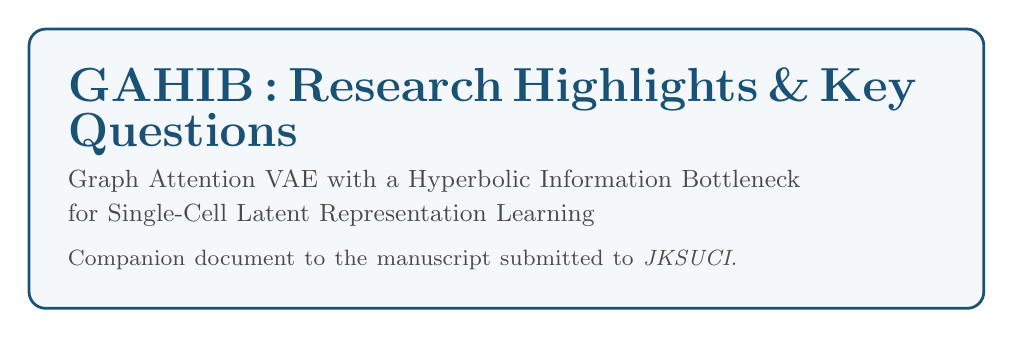
\begin{tikzpicture}
  \node[
    inner sep=14pt,
    text width=\linewidth-28pt,
    fill=softmist,
    draw=accentblue,
    line width=1.0pt,
    rounded corners=6pt
  ] {%
    {\LARGE\bfseries\color{accentblue}%
      GAHIB\,:\ Research Highlights \&\ Key Questions}\\[4pt]
    {\small\color{darkgray}%
      Graph Attention VAE with a Hyperbolic Information Bottleneck\\
      for Single-Cell Latent Representation Learning}\\[4pt]
    {\footnotesize\color{darkgray}%
      Companion document to the manuscript submitted to
      \textit{JKSUCI}.}%
  };
\end{tikzpicture}
\vspace{8pt}

% ── Research Highlights ───────────────────────────────────────────────────
\section*{Research Highlights}

\noindent
\small The five bullets below summarise the manuscript's central findings
and the evidence supporting each.\normalsize
\vspace{4pt}

\hlcard{plum}{1}{A unified hyperbolic single-cell VAE.}%
{GAHIB couples a graph-attention (GAT) encoder, a 2D information
 bottleneck, and a Lorentz-hyperbolic geometry loss inside a single
 variational objective --- to our knowledge the first framework to
 jointly optimise all three inductive biases for scRNA-seq.}

\hlcard{deepteal}{2}{Benchmarked at scale with statistical rigour.}%
{Eleven experimental studies on 53 scRNA-seq datasets, evaluated on
 20 metrics against 7 deep-learning, 5 classical dimensionality-reduction,
 5 geometric-VAE, and 4 disentanglement baselines. GAHIB matches or
 exceeds every baseline family, with BH-corrected significant gains
 over the majority of pairwise comparisons under paired Wilcoxon
 signed-rank tests.}

\hlcard{sunstone}{3}{Hyperbolic radii recover developmental hierarchy.}%
{On datasets with lineage annotations, Lorentz norms correlate with
 developmental order ($\rho_{s}=0.329$ mean, up to $0.673$ in enriched
 contexts; moderate effect), and the resulting pseudotime tracks
 diffusion pseudotime --- recovered \emph{without supervision}.}

\hlcard{coral}{4}{Latent dimensions encode tissue-specific biology.}%
{Tissue-specific GO Biological Process enrichment across four tissue
 contexts confirms that each latent dimension encodes biologically
 coherent, context-dependent programmes (adj.\ $p$ down to $10^{-23}$),
 with no off-tissue leakage.}

\hlcard{accentblue}{5}{Reproducible, robust, and practical.}%
{Multi-seed runs show $<$3\% standard deviation across all metrics;
 robustness sweeps show NMI spread $\leq 0.044$ across wide
 hyperparameter ranges; at fixed 200 epochs, training time is flat
 with cell count under fixed subgraph sampling.}

% ── Key Questions ─────────────────────────────────────────────────────────
\section*{Key Questions Addressed by This Work}

\noindent
\small
Our research programme was driven by five interlocking questions.
Each card below states the question and sketches the evidence the
manuscript provides in response.
\normalsize
\vspace{4pt}

\qcard{1}{Can graph attention and hyperbolic geometry be jointly
  optimised inside a single VAE, and does their synergy exceed the sum
  of its parts?}%
{Existing single-cell VAEs either use MLP encoders (ignoring
 cell-graph topology) or explore hyperbolic latent spaces (without
 neighbourhood-aware encoding). GAHIB is the first framework to
 simultaneously couple a GAT encoder, a 2D information bottleneck, and
 a Lorentz-hyperbolic geometry loss. A component ablation across 53
 datasets shows the full model statistically outperforms every partial
 configuration ($p<0.05$, paired Wilcoxon signed-rank, BH-corrected),
 confirming the three components are synergistic.}

\qcard{2}{Does hyperbolic latent geometry genuinely capture
  developmental hierarchy without explicit supervision?}%
{Lorentz norms learned by GAHIB align with known differentiation
 stages ($\rho_{s}=0.329$ mean, reaching $0.673$ in enriched contexts),
 producing emergent stemness scores. Pseudotime reconstructed from
 these norms tracks scanpy's diffusion pseudotime and is validated
 directly from the underlying gene expression via top $\pm$-correlated
 HVGs.}

\qcard{3}{How does GAHIB compare with leading deep-learning,
  classical, and geometric-VAE baselines?}%
{Eleven experimental studies --- seven comparative benchmarks against
 7 deep-learning, 5 classical DR, 5 geometric-VAE, and 4
 disentanglement baselines, plus four robustness/efficiency studies
 --- were conducted on 53 datasets across 6 tissue contexts and 20
 evaluation metrics. GAHIB delivers the strongest overall clustering
 and dimensionality-reduction fidelity with statistically significant
 gains over the majority of baselines.}

\qcard{4}{Are the learned latent dimensions biologically
  interpretable, and do they capture tissue-specific gene programmes?}%
{Decoder-Jacobian analysis recovers 31.5\% of known marker genes on
 representative datasets. Critically, GO Biological Process enrichment
 across four tissue contexts (dentate gyrus, hematopoiesis, Setty
 HSPC, hESC) shows individual latent dimensions encode distinct,
 tissue-specific programmes --- without any supervised gene-set input
 during training, and without off-tissue leakage.}

\qcard{5}{Is the method reproducible, robust, and computationally
  practical?}%
{Multi-seed experiments (5 runs $\times$ 53 datasets) show $<$3\%
 standard deviation across all metrics. Hyperparameter-sensitivity
 analysis confirms stable performance across wide ranges of
 bottleneck, Lorentz, and KL coefficients. At 200 epochs the
 per-dataset training time is flat with cell count under fixed
 subgraph sampling, and requires only a single GPU.}

% ── Closing note ─────────────────────────────────────────────────────────
\vspace{6pt}
\noindent
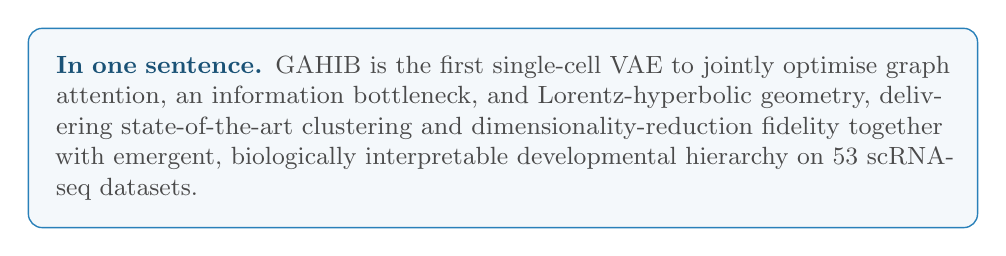
\begin{tikzpicture}
  \node[
    inner sep=10pt,
    text width=\linewidth-22pt,
    fill=softmist,
    draw=ruleblue,
    line width=0.5pt,
    rounded corners=5pt,
    font=\small\color{darkgray}
  ] {%
    \textbf{\color{accentblue}In one sentence.}\enspace
    GAHIB is the first single-cell VAE to jointly optimise graph
    attention, an information bottleneck, and Lorentz-hyperbolic
    geometry, delivering state-of-the-art clustering and
    dimensionality-reduction fidelity together with emergent,
    biologically interpretable developmental hierarchy on 53 scRNA-seq
    datasets.%
  };
\end{tikzpicture}

\end{document}
